%%%%%%%%%%%%%%%%%%%%%%%%%%%%%%%%%%%%%%%%%
% Short Sectioned Assignment
% LaTeX Template
% Version 1.0 (5/5/12)
%
% This template has been downloaded from:
% http://www.LaTeXTemplates.com
%
% Original author:
% Frits Wenneker (http://www.howtotex.com)
%
% License:
% CC BY-NC-SA 3.0 (http://creativecommons.org/licenses/by-nc-sa/3.0/)
%
%%%%%%%%%%%%%%%%%%%%%%%%%%%%%%%%%%%%%%%%%

%----------------------------------------------------------------------------------------
%	PACKAGES AND OTHER DOCUMENT CONFIGURATIONS
%----------------------------------------------------------------------------------------

\documentclass[paper=a4, fontsize=11pt]{scrartcl} % A4 paper and 11pt font size

\usepackage[T1]{fontenc} % Use 8-bit encoding that has 256 glyphs
\usepackage{fourier} % Use the Adobe Utopia font for the document - comment this line to return to the LaTeX default
\usepackage[english]{babel} % English language/hyphenation
\usepackage{amsmath,amsfonts,amsthm} % Math packages

\usepackage{lipsum} % Used for inserting dummy 'Lorem ipsum' text into the template

\usepackage{sectsty} % Allows customizing section commands
\allsectionsfont{\centering \normalfont\scshape} % Make all sections centered, the default font and small caps

\usepackage{fancyhdr} % Custom headers and footers

% my packages
\usepackage{commath}
\usepackage{mathtools}
\usepackage{graphicx}
\usepackage{algorithm}
\usepackage[]{algpseudocode}
\DeclarePairedDelimiter{\ceil}{\lceil}{\rceil}
\usepackage{pgfplots}
\pgfplotsset{compat=newest}
\usepackage{hyperref}
\usepackage{enumitem}
\usepackage{subcaption}
\usepackage{multirow}
\usepackage{tkz-graph}
\usepackage{adjustbox}
\usepackage{cancel}

\newlist{filedescription}{description}{2}
\setlist[filedescription]{font=\normalfont\normalcolor\bfseries\itshape}

\newlist{paramdescription}{description}{1}
\setlist[paramdescription]{font=\normalfont\normalcolor\itshape}

\pagestyle{fancyplain} % Makes all pages in the document conform to the custom headers and footers
\fancyhead{} % No page header - if you want one, create it in the same way as the footers below
\fancyfoot[L]{} % Empty left footer
\fancyfoot[C]{} % Empty center footer
\fancyfoot[R]{\thepage} % Page numbering for right footer
\renewcommand{\headrulewidth}{0pt} % Remove header underlines
\renewcommand{\footrulewidth}{0pt} % Remove footer underlines
\setlength{\headheight}{13.6pt} % Customize the height of the header

\numberwithin{equation}{section} % Number equations within sections (i.e. 1.1, 1.2, 2.1, 2.2 instead of 1, 2, 3, 4)
\numberwithin{figure}{section} % Number figures within sections (i.e. 1.1, 1.2, 2.1, 2.2 instead of 1, 2, 3, 4)
\numberwithin{table}{section} % Number tables within sections (i.e. 1.1, 1.2, 2.1, 2.2 instead of 1, 2, 3, 4)

\setlength\parindent{0pt} % Removes all indentation from paragraphs - comment this line for an assignment with lots of text

% new commands
\newcommand{\filename}[1]{\textbf{\textit{#1}}}
\newcommand{\funcname}[1]{\textbf{#1}}
\newcommand{\inv}{^{\raisebox{.2ex}{$\scriptscriptstyle-1$}}}
\renewcommand{\vec}[1]{\mathbf{#1}}

\makeatletter
\renewcommand*\env@matrix[1][*\c@MaxMatrixCols c]{%
  \hskip -\arraycolsep
  \let\@ifnextchar\new@ifnextchar
  \array{#1}}
\makeatother

\makeatletter
\def\BState{\State\hskip-\ALG@thistlm}
\makeatother

\DeclareMathOperator*{\argmin}{arg\,min} % Jan Hlavacek

%----------------------------------------------------------------------------------------
%	TITLE SECTION
%----------------------------------------------------------------------------------------

\newcommand{\horrule}[1]{\rule{\linewidth}{#1}} % Create horizontal rule command with 1 argument of height

\title{	
\normalfont \normalsize 
\textsc{Mathematical foundations of computer graphics and vision} \\ [25pt] % Your university, school and/or department name(s)
\horrule{0.5pt} \\[0.4cm] % Thin top horizontal rule
\huge Exercise 4. Sampling Patterns and Graph Cuts\\ % The assignment title
\horrule{2pt} \\[0.5cm] % Thick bottom horizontal rule
}

\author{Dongho Kang \\ \small 16-948-598} % Your name

\date{\normalsize May 7, 2017} % Today's date or a custom date

\begin{document}

\maketitle % Print the title

%----------------------------------------------------------------------------------------
%	README
%----------------------------------------------------------------------------------------

MATLAB R2016b version was used for coding and testing:

\begin{center}
MathWorks, MATLAB R2016b (9.1.0.441655) \\
64-bit (maci64) 
\end{center}

The \filename{code} directory contains the followings:

\begin{filedescription}
	\item [part1\_1.m] script .m file for exercise part 1.1.
	\item [part1\_2.m] script .m file for exercise part 1.2.
	\item [part2\_1.m] script .m file for exercise part 2.1. 
	\item [part2\_2.m] script .m file for exercise part 2.2. 
	\item [PART I] provided directory for part 1.
	\item [PART II] directory which contains implementation of part 2 and provided files including skeleton code etc.
	\item [?] TODO for testing part 2.2   
	\item [result] result image of part 1 and part 2.
		\begin{filedescription}
			\item [periodogram.png] TODO
			\item [pcf.png]			TODO
		\end{filedescription} 
\end{filedescription}

TOOD
For running each .m script, check dependencies (especially for \filename{part1\_4.m} and \filename{part1\_5.m}) and adjust parameters first. Note that \textbf{these scripts only work properly in MATLAB R2016b environment.} More details are stated in the \textit{Running} section of each parts.

%----------------------------------------------------------------------------------------
%	PROBLEM 1
%----------------------------------------------------------------------------------------

\section{exercise part 1: Analyzing Sampling Patterns}

In this exercise, two analysis techniques for sampling distributions was implemented:

\begin{enumerate}
	\item Periodogram (task 1)
	\item Pair Correlation Functions (task 2)
\end{enumerate}

%----------------------------------------------------------------------------------------
%	PERIODOGRAMS
%----------------------------------------------------------------------------------------
\subsection{Task 1: Computing periodograms of sampling patterns}

%----------------------------------------------------------------------------------------
\subsubsection{Description}

The periodogram is computed by \textbf{taking the Fourier transform of the impulse process corresponding to the sampling pattern.} It can be estimated by follows:

\begin{equation}
	P(w) = \abs{ \mathcal{F} [\frac{1}{n} \sum_{i=1}^{n} \delta(\vec{x} - \vec{x_i})]}^2
\end{equation}

where $\delta$ is the Dirac delta function, $\vec{x_i}$ are the locations of the points in a given points distribution and $\mathcal{F}$ denotes the Fourier transform. As suggested, this was implemented by rasterizing the function $\frac{1}{n} \sum_{i=1}^{n} \delta(\vec{x} - \vec{x_i})$ and taking the discrete Fourier transform by using MATLAB function \funcname{fft2}. 
\\

The periodogram was generated for the 4 different sampling algorithm, \textit{Matern, FPO, Dart, Balzer} and for each algorithm, results from 10 different point set were averaged.  

%----------------------------------------------------------------------------------------
\subsubsection{Running}

Run the script \filename{part1\_1.m} after setting the parameter \textit{width, height} for width and height of initial image. The default values are 400 for both \textit{width} and \textit{height}.

%----------------------------------------------------------------------------------------
\subsubsection{Result}

The Figure 1.1 is averaged periodograms of different sampling algorithms. In order to get a clear result image, the periodogram was scaled by 200.

\begin{figure}[H]
\caption{Averaged periodograms for the Matern, FPO, Dart and Balzer algorithms\label{fig:simple}}
\noindent\makebox[\textwidth]{
  \includegraphics[width=\textwidth]{periodogram-mean.png}
}
\end{figure}

%----------------------------------------------------------------------------------------
%	PAIR CORRELATION FUNCTION
%----------------------------------------------------------------------------------------
\subsection{Task 2: Computing the pair correlation function of sampling patterns}

%----------------------------------------------------------------------------------------
\subsubsection{Description}

Another way to analyze point distribution is via point process statistics. Pair correlation function (PCF) is widely accepted as the most informative. This measure $g(\vec{x}, \vec{y})$ describes the joint probability of having points at locations $\vec{x}$, and $\vec{y}$ at the same time. 
\\

In the isotropic case, PCF is only depends on the distance between the points and can be estimated as follows:

\begin{equation}
	\hat{g}(r) = \frac{\abs{V}}{\abs{\partial V_d} r^{d-1} n^2} \sum_{i \neq j} k_\sigma (r - d(\vec{x_i}, \vec{x_j}))
\end{equation}

Here $n$ is the number of samples and $\abs{\partial V_d}$ denotes the volume of the boundary of a unit sphere in a $d$ dimensional domain. Since it's 2-dimensional case, $d = 2$, $\abs{V} = 1$, $\abs{\partial V_d} = 2 \pi$ and $d(\vec{x_i}, \vec{x_j})$ is euclidean distance. The Gaussian kernel was used for $k_\sigma(x) = \frac{1}{\sqrt{\pi} \sigma} e^{-x^2 / \sigma^2}$. For the parameters, as suggested in the manual, $\sigma = 0.25$ was used. \\

\textbf{The most tricky part is choosing $r_a$, $r_b$ and normalizing the data}. $r_a$ and $r_b$ are the lower and upper limit of the $r$ values. In order to define these parameters in relative terms, sample points should be normalized by the distance $r_{max}$ defined as the minimum distance between pairs of points for the maximum packing of points in a given volume. (TODO REFERENCE) Two methods can be adapted for determining the $r_{max}$ value as follows:

\begin{itemize}
	\item the method by Lagae and Dutr\'{e} (TODO REFERENCE):
	\begin{equation}
		r_{max} = \sqrt{\frac{1}{2\sqrt{3} N}}
	\end{equation}
	
	where N is the number of samples. For $N = 1024$, $r_{max} = 0.0168$.
	
	\item the method by Gamito and Maddock (TODO REFERENCE): 
	\begin{equation}
		r_{max} = \sqrt[n]{\frac{\gamma_{n_{max}}}{N} \frac{\Gamma(\frac{n}{2} + 1)}{\pi^{n/2}}}
	\end{equation}  
	
	where N is the number of samples, $\Gamma$ denotes Gamma function, and finally $n = 2$, $\gamma_{n_{max}} = \frac{1}{6} \pi \sqrt{3}$ for 2-dimensional case. In fact, since $\Gamma(2) = 1$ for $n = 2$, $r_{max}$ is exactly same as $r_max$ calculated by Lagae and Dutr\'{e} method.
\end{itemize}

\textbf{As normalizing the samples by dividing by $r_{max}$, $\abs{V}$ also should be divided by $r_{max}^2$.} For the best value of $r_a$ and $r_b$, $r_a = 0.01 \sigma$, $r_b = 5$ were suggested but here $r_a = 2 \sigma$, $r_b = 10$ were used because of the numerical issue. 

%----------------------------------------------------------------------------------------
\subsubsection{Running}

Run the script \filename{part1\_2.m} after setting the parameter \textit{array\_size} for the number of $r$ values. Since every parameter was carefully chosen, do not change any value except \textit{array\_size}.

%----------------------------------------------------------------------------------------
\subsubsection{Result}

The Figure 1.2 is PCF of different sampling algorithms. The first datasets (\filename{<algorithm>/1.txt}) for each algorithm were used as sample data.

\begin{figure}[H]
\caption{PCF for the Matern, FPO, Dart and Balzer algorithms\label{fig:simple}}
\noindent\makebox[\textwidth]{
  \includegraphics[width=\textwidth]{pcf.png}
}
\end{figure}


%----------------------------------------------------------------------------------------
%	Discussion
%----------------------------------------------------------------------------------------
\subsection{Discussion}

\begin{itemize}
	\item Why we had to average over multiple point sets for each algorithm when computing the periodograms but not when computing the PCF's?
	
	\begin{figure}[H]
	\caption{The given graphical model for task 1.\label{fig:simple}}
	\noindent\makebox[\textwidth]{
			\includegraphics[width=\textwidth]{periodogram-1.png}
	}
	\end{figure}
	
	TODO
	
	\item Is the PCF are sufficient to describe the provided point patterns as they are only one dimensional, while the periodograms are two dimensional? Do the periodograms contain more information for the provided patters?
\end{itemize}

%----------------------------------------------------------------------------------------
%	PROBLEM 2
%----------------------------------------------------------------------------------------

\section{exercise part 2: Image Deformation Using Moving Least Squares}


%----------------------------------------------------------------------------------------
%	Handling max flow
%----------------------------------------------------------------------------------------
\subsection{Task 1: Handling max flow}

\subsubsection{Description}

\begin{figure}[H]
\caption{The given graphical model for task 1.\label{fig:simple}}
\vspace*{5mm}
\centering
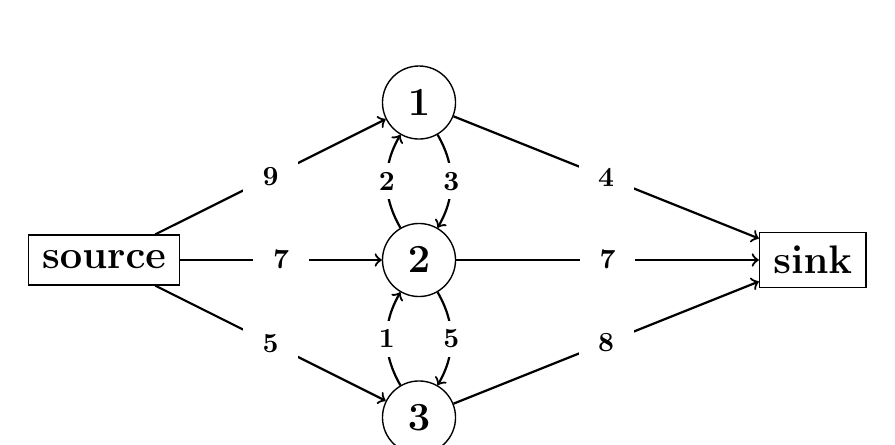
\begin{tikzpicture}
	\GraphInit[vstyle = Dijkstra]
	\tikzset{
	  LabelStyle/.style = { minimum width = 2em, font = \bfseries },
	  VertexStyle/.append style = { inner sep=5pt,
	                                font = \Large\bfseries},
	  EdgeStyle/.append style = {->} }
%	\draw[help lines] (-2, -2) grid (2, 2);
	\SetGraphUnit{2}
	\Vertex{2}
	\begin{scope}[VertexStyle/.append style = {inner sep = 5pt,
                                           shape=rectangle}]
	\EA[unit=5](2){sink}
	\WE[unit=4](2){source}
	\end{scope}
	\NO[unit=2](2){1}
	\SO[unit=2](2){3}
	\Edge[label = 9](source)(1)
	\Edge[label = 7](source)(2)
	\Edge[label = 5](source)(3)
	\Edge[label = 3, style={bend left}](1)(2)
	\Edge[label = 2, style={bend left}](2)(1)
	\Edge[label = 1, style={bend left}](3)(2)
	\Edge[label = 5, style={bend left}](2)(3)
	\Edge[label = 4](1)(sink)
	\Edge[label = 7](2)(sink)
	\Edge[label = 8](3)(sink)
\end{tikzpicture}
\end{figure}

The max flow problem for Figure 2.1 was solved by the algorithm by Boykov and Kolmogorov (BK algorithm). It was implemented by using \textit{BK library}. The comparison between the result by the algorithm and result by hand is discussed in the section 2.1.4.
\\

For unary costs (edges to source and sink) and pairwise costs (edges between nodes), following values were set as input. 

(TODO TABLE - unary cost)

(TODO TABLE - pairwise cost)


%----------------------------------------------------------------------------------------
\subsubsection{Running}

Since third party library \textit{BK library} was used, check if the library was built properly. All library files including \filename{bin} directory which contains the compiled binaries, should be placed in the \filename{PART II/GraphCut} directory. \\

Run the script \filename{part2\_1.m}. The script invoke subscript \filename{PART II/task1.m}, the implementation of computing max flow of Figure 2.1. 

%----------------------------------------------------------------------------------------
\subsubsection{Result}

The result of the max flow by BK algorithm as follows:

\begin{figure}[H]
\caption{The given graphical model for task 1.\label{fig:simple}}
\vspace*{5mm}
\centering
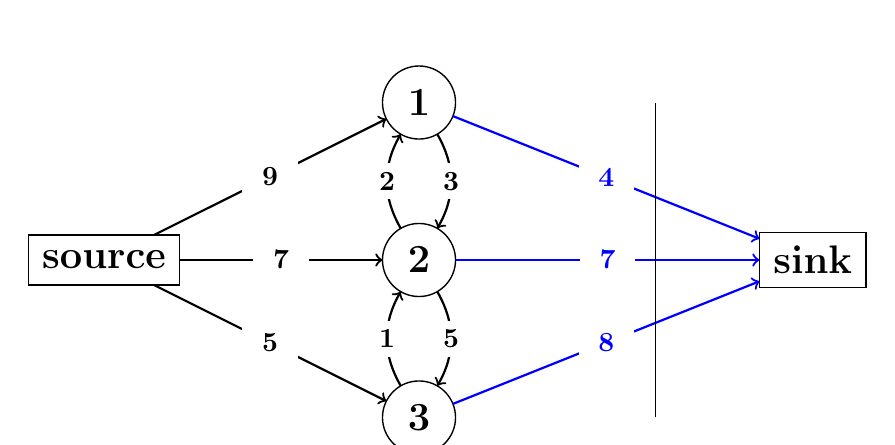
\begin{tikzpicture}
	\tikzset{
	  LabelStyle/.style = { minimum width = 2em, font = \bfseries },
	  VertexStyle/.append style = { inner sep=5pt,
	                                font = \Large\bfseries},
	  EdgeStyle/.append style = {->} }
	\SetGraphUnit{2}
	\Vertex{2}
	\begin{scope}[VertexStyle/.append style = {inner sep = 5pt,
                                           shape=rectangle}]
	\EA[unit=5](2){sink}
	\WE[unit=4](2){source}
	\end{scope}
	\NO[unit=2](2){1}
	\SO[unit=2](2){3}
	\Edge[label = 9](source)(1)
	\Edge[label = 7](source)(2)
	\Edge[label = 5](source)(3)
	\Edge[label = 3, style={bend left}](1)(2)
	\Edge[label = 2, style={bend left}](2)(1)
	\Edge[label = 1, style={bend left}](3)(2)
	\Edge[label = 5, style={bend left}](2)(3)
	\Edge[label = 4, style={blue}, labeltext=blue](1)(sink)
	\Edge[label = 7, style={blue}, labeltext=blue](2)(sink)
	\Edge[label = 8, style={blue}, labeltext=blue](3)(sink)
	\draw (3,-2) -- (3,2);
\end{tikzpicture}
\end{figure}

\begin{itemize}
	\item max flow (or min cut energy) $= 19$ 
	\item label 1 was assigned to all nodes i.e. nodes are connected with source. 
\end{itemize}

%----------------------------------------------------------------------------------------
\subsubsection{Discussion}

Steps for computing max flow by hand is as follows:

\begin{figure}[H]
\caption{The given graphical model for task 1.\label{fig:simple}}
\vspace*{5mm}
\centering
\begin{subfigure}[b]{0.4\textwidth}
	\begin{adjustbox}{width=\textwidth}
		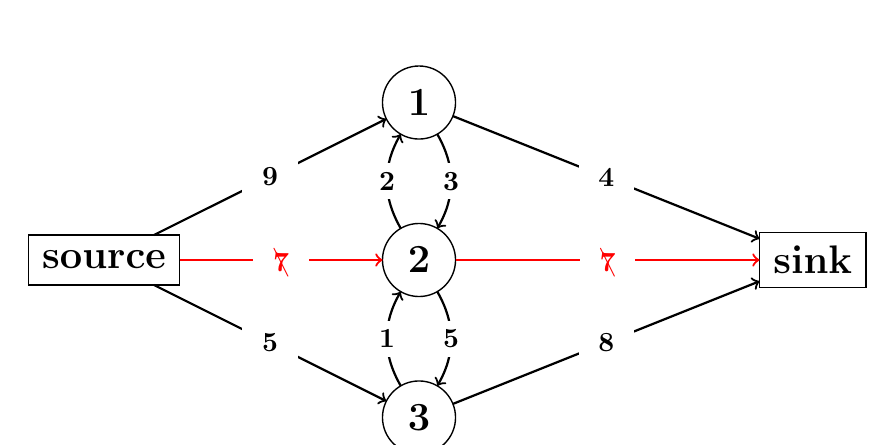
\begin{tikzpicture}
%			\GraphInit[vstyle = Dijkstra]
			\tikzset{
			  LabelStyle/.style = { minimum width = 2em, font = \bfseries },
			  VertexStyle/.append style = { inner sep=5pt,
			                                font = \Large\bfseries},
			  EdgeStyle/.append style = {->} }
			\SetGraphUnit{2}
			\Vertex{2}
			\begin{scope}[VertexStyle/.append style = {inner sep = 5pt,
		                                           shape=rectangle}]
			\EA[unit=5](2){sink}
			\WE[unit=4](2){source}
			\end{scope}
			\NO[unit=2](2){1}
			\SO[unit=2](2){3}
			\Edge[label = 9](source)(1)
			\Edge[label = \bcancel{7}, style=red, labeltext=red](source)(2)
			\Edge[label = 5](source)(3)
			\Edge[label = 3, style={bend left}](1)(2)
			\Edge[label = 2, style={bend left}](2)(1)
			\Edge[label = 1, style={bend left}](3)(2)
			\Edge[label = 5, style={bend left}](2)(3)
			\Edge[label = 4](1)(sink)
			\Edge[label = \bcancel{7}, style=red, labeltext=red](2)(sink)
			\Edge[label = 8](3)(sink)
		\end{tikzpicture}
	\end{adjustbox}	
	\caption{flow $= 7$}
\end{subfigure}
\vspace*{10mm}
\hspace*{10mm}
\begin{subfigure}[b]{0.4\textwidth}
	\begin{adjustbox}{width=1.0\textwidth}
		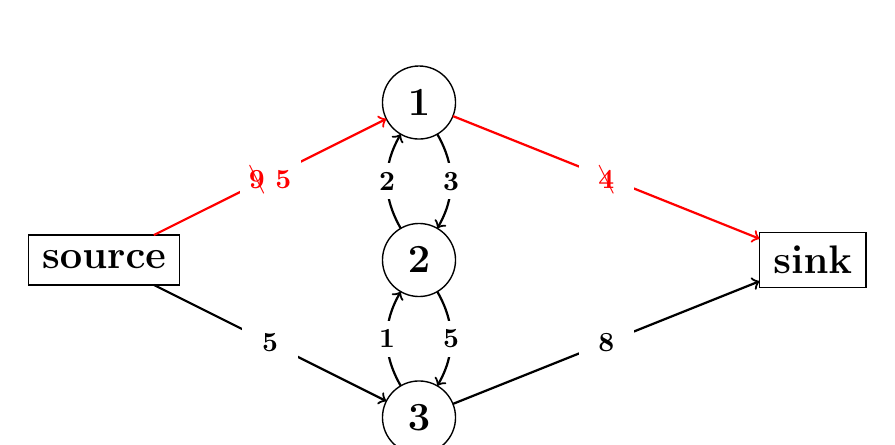
\begin{tikzpicture}
%			\GraphInit[vstyle = Dijkstra]
			\tikzset{
			  LabelStyle/.style = { minimum width = 2em, font = \bfseries },
			  VertexStyle/.append style = { inner sep=5pt,
			                                font = \Large\bfseries},
			  EdgeStyle/.append style = {->} }
			\SetGraphUnit{2}
			\Vertex{2}
			\begin{scope}[VertexStyle/.append style = {inner sep = 5pt,
		                                           shape=rectangle}]
			\EA[unit=5](2){sink}
			\WE[unit=4](2){source}
			\end{scope}
			\NO[unit=2](2){1}
			\SO[unit=2](2){3}
			\Edge[label = \bcancel{9} 5, style=red, labeltext=red](source)(1)
			\Edge[label = 5](source)(3)
			\Edge[label = 3, style={bend left}](1)(2)
			\Edge[label = 2, style={bend left}](2)(1)
			\Edge[label = 1, style={bend left}](3)(2)
			\Edge[label = 5, style={bend left}](2)(3)
			\Edge[label = \bcancel{4}, style=red, labeltext=red](1)(sink)
			\Edge[label = 8](3)(sink)
		\end{tikzpicture}
	\end{adjustbox}	
	\caption{flow $= 11$}
\end{subfigure}
\begin{subfigure}[b]{0.4\textwidth}
	\begin{adjustbox}{width=\textwidth}
		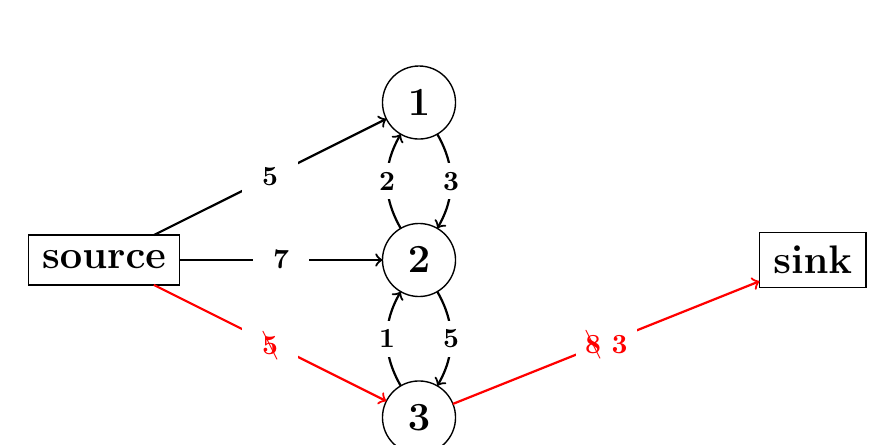
\begin{tikzpicture}
%			\GraphInit[vstyle = Dijkstra]
			\tikzset{
			  LabelStyle/.style = { minimum width = 2em, font = \bfseries },
			  VertexStyle/.append style = { inner sep=5pt,
			                                font = \Large\bfseries},
			  EdgeStyle/.append style = {->} }
			\SetGraphUnit{2}
			\Vertex{2}
			\begin{scope}[VertexStyle/.append style = {inner sep = 5pt,
		                                           shape=rectangle}]
			\EA[unit=5](2){sink}
			\WE[unit=4](2){source}
			\end{scope}
			\NO[unit=2](2){1}
			\SO[unit=2](2){3}
			\Edge[label = 5](source)(1)
			\Edge[label = 7](source)(2)
			\Edge[label = \bcancel{5}, style=red, labeltext=red](source)(3)
			\Edge[label = 3, style={bend left}](1)(2)
			\Edge[label = 2, style={bend left}](2)(1)
			\Edge[label = 1, style={bend left}](3)(2)
			\Edge[label = 5, style={bend left}](2)(3)
			\Edge[label = \bcancel{8} 3, style=red, labeltext=red](3)(sink)
		\end{tikzpicture}
	\end{adjustbox}	
	\caption{flow $= 16$}
\end{subfigure}
\vspace*{10mm}
\hspace*{10mm}
\begin{subfigure}[b]{0.4\textwidth}
	\begin{adjustbox}{width=1.0\textwidth}
		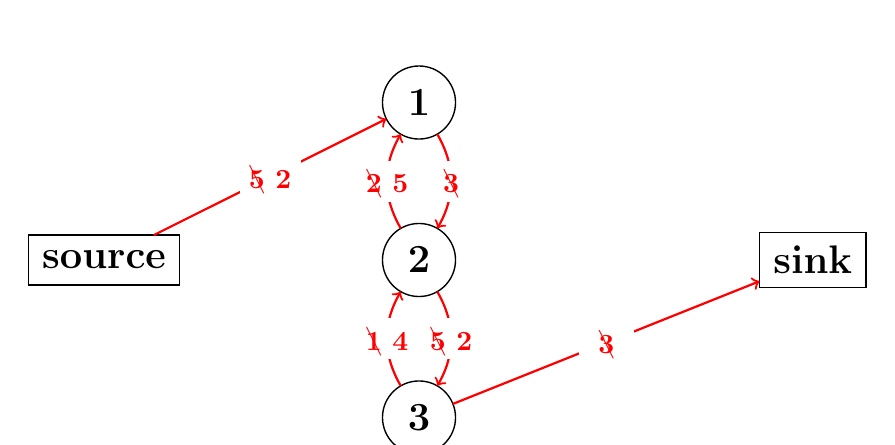
\begin{tikzpicture}
%			\GraphInit[vstyle = Dijkstra]
			\tikzset{
			  LabelStyle/.style = { minimum width = 2em, font = \bfseries },
			  VertexStyle/.append style = { inner sep=5pt,
			                                font = \Large\bfseries},
			  EdgeStyle/.append style = {->} }
			\SetGraphUnit{2}
			\Vertex{2}
			\begin{scope}[VertexStyle/.append style = {inner sep = 5pt,
		                                           shape=rectangle}]
			\EA[unit=5](2){sink}
			\WE[unit=4](2){source}
			\end{scope}
			\NO[unit=2](2){1}
			\SO[unit=2](2){3}
			\Edge[label = \bcancel{5} 2, style=red, labeltext=red](source)(1)
			\Edge[label = \bcancel{3}, style={red, bend left}, labeltext=red](1)(2)
			\Edge[label = \bcancel{2} 5, style={red, bend left}, labeltext=red](2)(1)
			\Edge[label = \bcancel{1} 4, style={red, bend left}, labeltext=red](3)(2)
			\Edge[label = \bcancel{5} 2, style={red, bend left}, labeltext=red](2)(3)
			\Edge[label = \bcancel{3}, style=red, labeltext=red](3)(sink)
		\end{tikzpicture}
	\end{adjustbox}	
	\caption{flow $= 19$}
\end{subfigure}
\begin{subfigure}[b]{0.4\textwidth}
	\begin{adjustbox}{width=\textwidth}
		\begin{tikzpicture}
%			\GraphInit[vstyle = Dijkstra]
			\tikzset{
			  LabelStyle/.style = { minimum width = 2em, font = \bfseries },
			  VertexStyle/.append style = { inner sep=5pt,
			                                font = \Large\bfseries},
			  EdgeStyle/.append style = {->} }
			\SetGraphUnit{2}
			\Vertex{2}
			\begin{scope}[VertexStyle/.append style = {inner sep = 5pt,
		                                           shape=rectangle}]
			\EA[unit=5](2){sink}
			\WE[unit=4](2){source}
			\end{scope}
			\NO[unit=2](2){1}
			\SO[unit=2](2){3}
			\Edge[label = 2](source)(1)
			\Edge[label = 5, style={bend left}](2)(1)
			\Edge[label = 4, style={bend left}](3)(2)
			\Edge[label = 2, style={bend left}](2)(3)
		\end{tikzpicture}
	\end{adjustbox}	
	\caption{terminated with flow $= 19$}
\end{subfigure}
\vspace*{10mm}
\hspace*{10mm}
\begin{subfigure}[b]{0.4\textwidth}
	\begin{adjustbox}{width=1.0\textwidth}
		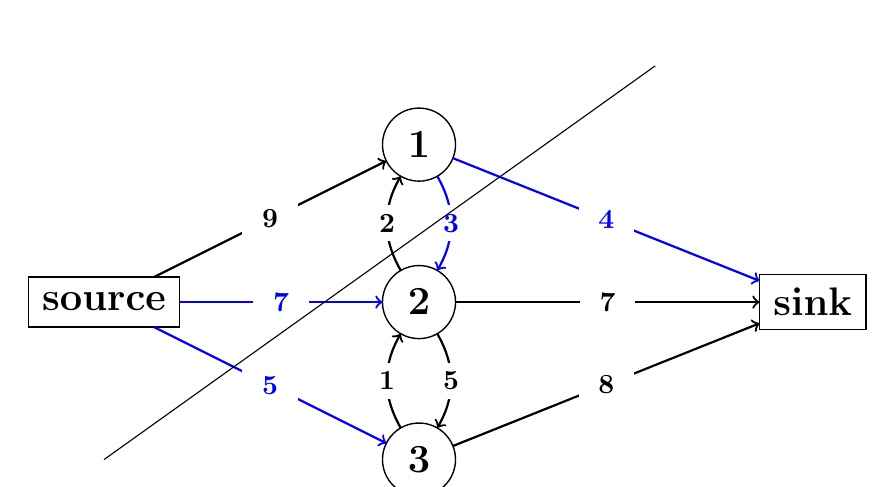
\begin{tikzpicture}
%			\GraphInit[vstyle = Dijkstra]
			\tikzset{
			  LabelStyle/.style = { minimum width = 2em, font = \bfseries },
			  VertexStyle/.append style = { inner sep=5pt,
			                                font = \Large\bfseries},
			  EdgeStyle/.append style = {->} }
			\SetGraphUnit{2}
			\Vertex{2}
			\begin{scope}[VertexStyle/.append style = {inner sep = 5pt,
		                                           shape=rectangle}]
			\EA[unit=5](2){sink}
			\WE[unit=4](2){source}
			\end{scope}
			\NO[unit=2](2){1}
			\SO[unit=2](2){3}
			\Edge[label = 9](source)(1)
			\Edge[label = 7, style={blue}, labeltext=blue](source)(2)
			\Edge[label = 5, style={blue}, labeltext=blue](source)(3)
			\Edge[label = 3, style={bend left, blue}, labeltext=blue](1)(2)
			\Edge[label = 2, style={bend left}](2)(1)
			\Edge[label = 1, style={bend left}](3)(2)
			\Edge[label = 5, style={bend left}](2)(3)
			\Edge[label = 4, style={blue}, labeltext=blue](1)(sink)
			\Edge[label = 7](2)(sink)
			\Edge[label = 8](3)(sink)
			\draw (-4,-2) -- (3,3);
		\end{tikzpicture}
	\end{adjustbox}	
	\caption{graph cut with cost $= 19$}
\end{subfigure}
\end{figure}

\begin{itemize}
	\item max flow (or min cut energy) $= 19$ 
	\item label 1 was assigned to node 1. Thus, node 1 is connected with source. 
	\item label 2 was assigned to node 2 and node 3. Thus, node 2 and node 3 are connected with sink. 
\end{itemize}

The result above is same in max flow with the result by BK algorithm but different in labelling. Both labelling is correct because cost of cutting is 19 in both cases.


%----------------------------------------------------------------------------------------
%	Interactive Segmentation
%----------------------------------------------------------------------------------------
\subsection{Task 2: Interactive Segmentation}

\subsubsection{Description}

\begin{enumerate}
	\item color histogram 
	\item getting unary cost
	\item getting pairwise cost
	\item building and solving a graph. segmentation 
	\item changing background using the obtained segmentation 
\end{enumerate}


\paragraph{Color histogram}

\paragraph{Unary cost}

\paragraph{Pairwise cost}

\paragraph{Graph and segmentation}

\paragraph{Changing background}

%----------------------------------------------------------------------------------------
\subsubsection{Running}

%----------------------------------------------------------------------------------------
\subsubsection{Result}

%----------------------------------------------------------------------------------------
\subsubsection{Discussion}

\end{document}